\documentclass[12pt,a4paper]{report}

\usepackage[utf8]{inputenc}
\usepackage[T1]{fontenc}
\usepackage[spanish,es-tabla]{babel}
\usepackage{lmodern}
\usepackage{microtype}
\usepackage{geometry}
\usepackage{xurl}
\usepackage{hyperref}
\usepackage{graphicx}
\usepackage{longtable}
\usepackage{tabularx}
\usepackage{array}
\usepackage{booktabs}
\usepackage{makecell}
\usepackage{ragged2e}
\usepackage{listings}
\usepackage{enumitem}
\usepackage{amsmath}
\usepackage{amssymb}
\usepackage{caption}
\usepackage{float}
\usepackage{placeins}
\usepackage{pdflscape}
\usepackage{xcolor}

\geometry{margin=2.5cm}
\hypersetup{
  colorlinks=true,
  linkcolor=blue!50!black,
  citecolor=blue!50!black,
  urlcolor=blue!50!black,
  pdftitle={Neo Angele Risk Lab},
  pdfauthor={Salazar Martínez Liam Antonio}
}

\setlist{itemsep=0.2em, topsep=0.4em}
\captionsetup{font=small,labelfont=bf}
\emergencystretch=3em

\definecolor{codegray}{RGB}{245,245,245}
\definecolor{codeborder}{RGB}{210,210,210}
\lstdefinelanguage{bash}{
  morekeywords={sudo,apt-get,install,update,upgrade,curl,echo,tee,git,cd,docker,compose,python,bash,if,then,elif,else,fi,for,do,done},
  sensitive=true,
  morecomment=[l]{\#},
  morestring=[b]",
  morestring=[b]'
}
\lstdefinestyle{neoange}{
  backgroundcolor=\color{codegray},
  basicstyle=\ttfamily\footnotesize,
  breakatwhitespace=false,
  breaklines=true,
  captionpos=b,
  columns=fullflexible,
  frame=single,
  framerule=0.3pt,
  rulecolor=\color{codeborder},
  keepspaces=true,
  numbers=left,
  numbersep=6pt,
  numberstyle=\tiny\color{gray},
  showstringspaces=false,
  tabsize=2
}
\lstset{style=neoange}

\newcommand{\code}[1]{\texttt{#1}}
\DeclareRobustCommand{\codeid}[1]{\texttt{\detokenize{#1}}}
\DeclareRobustCommand{\codepath}[1]{\texttt{\detokenize{#1}}}
\DeclareRobustCommand{\filepath}[1]{\nolinkurl{#1}}
\newcolumntype{Y}{>{\RaggedRight\arraybackslash}X}

\begin{document}

\begin{titlepage}
\centering
{\Large Desarrollo de Aplicaciones para Análisis de Datos\par}
\vspace{2.2cm}
{\Huge\bfseries Neo Angele Risk Lab\par}
\vspace{0.4cm}
{\Large Plataforma analítica explicable para análisis, priorización y simulación experimental de objetos cercanos a la Tierra\par}
\vspace{2.2cm}
{\large Autores\par}
{\Large Salazar Martínez Liam Antonio\par}
\vfill
{\large Repositorio público\par}
\url{https://github.com/LiamSalazar/NEO-Angele-Risk-Lab}\par
\vspace{1cm}
{\large Fecha de preparación: 21 de junio de 2026\par}
\end{titlepage}

\tableofcontents
\clearpage

\chapter{Resumen}

Neo Angele Risk Lab es una plataforma académica de ingeniería de datos, analítica explicable, simulación experimental y visualización para estudiar objetos cercanos a la Tierra, conocidos como NEO por sus siglas en inglés. El proyecto integra datos públicos de NASA/JPL, los preserva en una capa bronze, los normaliza con PySpark hacia silver, construye un dataset gold, calcula un \emph{Risk Priority Score} explicable, ejecuta simulaciones Monte Carlo del score, produce simulaciones orbitales aproximadas, construye un grafo orbital de similitud, entrena modelos tabulares y baselines de grafo, expone resultados mediante FastAPI y los presenta en un frontend React/Vite.

El problema que resuelve no es la predicción oficial de impactos. El sistema organiza fuentes públicas heterogéneas, hace trazable el flujo de datos, convierte campos astronómicos técnicos en indicadores interpretables y ofrece una interfaz para priorizar revisión experimental. El score principal es un ranking analítico interno de 0 a 100. La evidencia de machine learning y GNN se trata como evidencia secundaria, no como criterio oficial de riesgo ni como sustituto de NASA/JPL, CNEOS o Sentry.


\chapter{Introducción}

Los NEO son objetos pequeños del Sistema Solar cuyas órbitas se acercan a la región orbital terrestre. Su análisis combina identificación, propiedades físicas, elementos orbitales, acercamientos cercanos, calidad observacional y señales de sistemas especializados como Sentry. Aunque NASA/JPL ofrece interfaces públicas, los datos aparecen repartidos entre API con formatos, granularidades y finalidades distintas: SBDB Object describe objetos individuales, SBDB Query permite consultas tabulares, CAD aporta acercamientos cercanos y Sentry resume objetos con señales de impacto potencial dentro del sistema oficial.

Esta dispersión dificulta que estudiantes o usuarios técnicos sin experiencia previa construyan una lectura integrada. Una fila puede contener magnitud absoluta \code{h}, MOID, elementos orbitales, conteos de observaciones, fechas de acercamiento y campos Sentry, sin contexto, esos campos son difíciles de interpretar, entonces Neo Angele Risk Lab surge para centralizar esas fuentes, preservar trazabilidad, construir features reproducibles, priorizar objetos de manera explicable, simular sensibilidad y mostrar resultados en una aplicación web.

El proyecto se ubica en la asignatura Desarrollo de Aplicaciones para Análisis de Datos porque combina adquisición de datos, almacenamiento por capas, procesamiento con Spark, programación orientada a objetos, diseño de API, frontend, modelos de machine learning, grafo orbital, pruebas automatizadas y empaquetamiento con Docker.

\chapter{Objetivos}

\section{Objetivo General}

Diseñar, implementar y documentar una plataforma analítica reproducible para integrar datos públicos de objetos cercanos a la Tierra, construir features de riesgo experimental, priorizar objetos mediante un score explicable, simular incertidumbre, producir evidencia secundaria con modelos tabulares y de grafo, y visualizar resultados mediante una API y un frontend web.

\section{Objetivos Específicos}

\begin{enumerate}
  \item Ingerir datos de SBDB Object, SBDB Query, CAD y Sentry mediante clientes Python separados.
  \item Preservar respuestas crudas en una capa bronze con metadatos de origen y tiempo.
  \item Normalizar los datos con PySpark hacia tablas silver y construir un dataset gold de features analíticas.
  \item Representar el dominio NEO mediante clases Python con composición, agregados y objetos de valor.
  \item Calcular un \emph{Risk Priority Score} reproducible, explicable y versionado.
  \item Simular la sensibilidad del score mediante perturbaciones Monte Carlo y análisis determinista.
  \item Simular escenarios orbitales aproximados mediante clones, covarianza cuando esté disponible y fallback heurístico cuando no lo esté.
  \item Entrenar modelos tabulares y baselines de grafo para generar evidencia secundaria y auditar leakage.
  \item Construir un grafo orbital kNN para estudiar vecindarios de similitud.
  \item Exponer resultados mediante FastAPI y presentarlos en un frontend React/Vite.
  \item Documentar instalación, uso, resultados, limitaciones y reproducibilidad.
\end{enumerate}

\chapter{Justificación y Motivación}

El dominio NEO tiene valor académico porque conecta física orbital, ingeniería de datos, APIs públicas, incertidumbre, machine learning e interfaces explicables. La motivación principal es convertir datos dispersos en un laboratorio reproducible que pueda ser inspeccionado de extremo a extremo. El proyecto no intenta reemplazar cálculos profesionales, su utilidad está en unificar y hacer entendibles los datos sobre los riesgos asociados a los NEOs para gente fuera del área de datos o del dominio (astrofísica).

La justificación de PySpark y Parquet proviene del patrón de datos por capas. Aunque el dataset local no es masivo, Spark permite practicar un modelo de procesamiento distribuible, con esquemas y transformaciones declarativas. Parquet ofrece almacenamiento columnar eficiente y compatible con Pandas, Spark y herramientas analíticas.

La justificación del score explicable proviene de la necesidad de ordenar objetos para revisión, ya que una probabilidad oficial de impacto requiere efemérides, observación profesional y sistemas especializados, el proyecto no posee ni reclama esa capacidad, sin embargo, calcula un score experimental que combina tamaño, proximidad orbital, acercamientos, señal Sentry, incertidumbre y calidad de datos.

La justificación de ML/GNN es secundaria. Los modelos ayudan a comparar patrones, detectar desacuerdos y mostrar cómo cambia el desempeño según conjuntos de features con o sin variables cercanas a la definición PHA. Por esa razón se documenta el leakage y se separa el score principal de la evidencia aprendida.

\chapter{Marco Conceptual del Dominio NEO}

Un NEO es un objeto cuyo recorrido orbital lo acerca a la vecindad de la Tierra. Un PHA, \emph{Potentially Hazardous Asteroid}, es una etiqueta relacionada con criterios de tamaño y proximidad orbital; en términos prácticos suele estar asociada a magnitud absoluta y MOID. Un non-PHA es un objeto que no cumple esa etiqueta en el dataset usado.

MOID significa \emph{Minimum Orbit Intersection Distance}. No es una distancia observada en una fecha concreta, sino una medida geométrica de proximidad mínima entre dos órbitas. La magnitud absoluta \code{H} describe brillo intrínseco: valores menores suelen asociarse con objetos más grandes si se asume un albedo comparable. El diámetro y el albedo son propiedades físicas; cuando faltan, el sistema puede usar proxies derivados, siempre marcados como aproximaciones.

Los elementos orbitales clásicos incluyen semieje mayor \code{a}, excentricidad \code{e}, inclinación \code{i}, longitud del nodo ascendente \code{om}, argumento del perihelio \code{w}, anomalía media \code{ma}, movimiento medio \code{n}, periodo \code{per}, perihelio \code{q}, afelio \code{ad} y MOID. Un \emph{close approach} es un acercamiento registrado a un cuerpo, con distancia, velocidad relativa y fecha. Sentry es el sistema de monitoreo de riesgo de impacto de CNEOS/JPL y sus señales no equivalen al score experimental del proyecto.

La escala de Palermo y la escala de Torino son formas de comunicar riesgo de impacto en contextos oficiales. En este repositorio, \code{sentry\_ps\_cum}, \code{sentry\_ps\_max}, \code{sentry\_ts\_max}, \code{sentry\_ip} y \code{sentry\_n\_imp} se usan únicamente como señales disponibles cuando existen. La diferencia central es:

\begin{itemize}
  \item La etiqueta PHA describe una clasificación del objeto.
  \item Sentry describe una señal oficial externa cuando está presente.
  \item El \emph{Risk Priority Score} ordena revisión experimental dentro de Neo Angele Risk Lab.
\end{itemize}

\chapter{Fuentes de Datos}

El proyecto usa fuentes públicas NASA/JPL documentadas oficialmente \cite{jpl_sbdb,jpl_sbdb_query,jpl_cad,jpl_sentry}. La conexión con el pipeline aparece en \filepath{src/neo_ange/clients} y \filepath{src/neo_ange/pipelines/ingestion.py}.

\begin{longtable}{>{\RaggedRight\arraybackslash}p{0.20\linewidth}>{\RaggedRight\arraybackslash}p{0.26\linewidth}>{\RaggedRight\arraybackslash}p{0.26\linewidth}>{\RaggedRight\arraybackslash}p{0.18\linewidth}}
\caption{Fuentes de datos usadas por el proyecto.}\\
\toprule
Fuente & Aporta & Limitaciones & Cliente\\
\midrule
\endfirsthead
\toprule
Fuente & Aporta & Limitaciones & Cliente\\
\midrule
\endhead
SBDB Object API & Detalle por objeto, elementos orbitales, propiedades físicas y metadatos. & La disponibilidad de campos varía por objeto; la covarianza no siempre aparece en el gold local. & \code{SBDBObjectClient}\\
SBDB Query API & Consulta tabular de objetos y campos seleccionados. & Requiere seleccionar columnas y filtros; no reemplaza detalle objeto por objeto. & \code{SBDBQueryClient}\\
CAD API & Registros de acercamientos cercanos, distancias, velocidad y cuerpo. & Cobertura limitada por parámetros de consulta y horizonte. & \code{CloseApproachClient}\\
Sentry API & Señales de riesgo Sentry, probabilidades y campos Palermo/Torino cuando existen. & La ausencia de señal no significa riesgo cero; solo indica que no hay dato Sentry en el snapshot. & \code{SentryClient}\\
\bottomrule
\end{longtable}

\chapter{Diccionario de Datos}

El diccionario siguiente agrupa los campos principales que aparecen en el dataset gold y en los reportes. No inventa columnas: los nombres fueron verificados en \filepath{data/gold/neo_risk_features}, \filepath{data/gold/risk_scores}, \filepath{reports/model_evidence} y módulos de código.

{\footnotesize
\setlength{\tabcolsep}{3.5pt}
\begin{longtable}{>{\RaggedRight\arraybackslash}p{0.20\linewidth}>{\RaggedRight\arraybackslash}p{0.30\linewidth}>{\RaggedRight\arraybackslash}p{0.14\linewidth}>{\RaggedRight\arraybackslash}p{0.26\linewidth}}
\caption{Diccionario de datos resumido por grupo.}\\
\toprule
Campo & Significado & Fuente & Uso en el sistema\\
\midrule
\endfirsthead
\toprule
Campo & Significado & Fuente & Uso en el sistema\\
\midrule
\endhead
\code{object\_key}, \code{spkid}, \code{des}, \code{full\_name}, \code{name} & Identificadores técnicos y etiquetas humanas. & SBDB & \code{AsteroidIdentity}, búsqueda, API, frontend.\\
\code{neo}, \code{pha}, \code{orbit\_class\_code}, \code{orbit\_class\_name} & Clasificación orbital y etiqueta PHA. & SBDB & Objetivo ML, filtros, contexto de dominio.\\
\code{h}, \code{diameter}, \code{albedo}, \code{log\_diameter}, \code{size\_proxy\_score} & Brillo, tamaño y proxies físicos. & SBDB/gold & \code{PhysicalProperties}, score físico, modelos.\\
\code{e}, \code{a}, \code{q}, \code{i}, \code{om}, \code{w}, \code{ma}, \code{n}, \code{per}, \code{ad}, \code{moid}, \code{moid\_ld} & Elementos orbitales y proximidad geométrica. & SBDB/gold & \code{Orbit}, score orbital, grafo, simulación orbital.\\
\code{condition\_code}, \code{arc\_length}, \code{n\_obs\_used}, \code{rms}, \code{observation\_quality\_score}, \code{uncertainty\_proxy\_score} & Calidad observacional e incertidumbre aproximada. & SBDB/gold & Componente de incertidumbre, simulaciones, limitaciones.\\
\code{min\_close\_approach\_dist}, \code{min\_close\_approach\_dist\_min}, \code{max\_close\_approach\_v\_rel}, \code{next\_close\_approach\_datetime}, \code{close\_approach\_count} & Resumen de acercamientos. & CAD/gold & \code{CloseApproachSummary}, score de acercamiento, frontend.\\
\code{sentry\_flag}, \code{sentry\_ip}, \code{sentry\_ps\_cum}, \code{sentry\_ps\_max}, \code{sentry\_ts\_max}, \code{sentry\_n\_imp}, \code{sentry\_presence\_score} & Señales Sentry disponibles. & Sentry/gold & \code{SentryRiskSignal}, componente Sentry, explicación.\\
\code{risk\_score}, \code{risk\_score\_0\_100}, componentes y \code{risk\_category} & Score experimental, versión normalizada y banda. & \code{RiskScorer} & Ranking, API, frontend, simulaciones.\\
\code{mean\_score}, \code{std\_score}, \code{p05\_score}, \code{median\_score}, \code{p95\_score}, \code{probability\_score\_above\_60}, \code{category\_shift\_probability} & Estadísticos Monte Carlo del score. & \code{MonteCarloEngine} & Página de Score Simulation y findings.\\
\code{n\_clones}, \code{valid\_clone\_count}, \code{dispersion\_index}, \code{scenario\_category}, \code{simulation\_method}, \code{covariance\_available}, \code{cad\_validation\_error\_au} & Métricas de clones orbitales. & \code{OrbitalMonteCarloEngine} & Página de Orbital Simulation y reportes.\\
\code{model\_name}, \code{feature\_set}, \code{predicted\_probability}, \code{confidence\_bucket}, \code{leakage\_risk}, \code{evidence\_role} & Evidencia ML/GNN por objeto. & \code{ModelEvidenceBuilder} & Model evidence, desacuerdos, frontend.\\
\bottomrule
\end{longtable}
}

\chapter{Arquitectura General del Sistema}

El flujo real del proyecto sigue la cadena:

\[
\text{NASA/JPL APIs}
\rightarrow \text{clients}
\rightarrow \text{ingestion}
\rightarrow \text{bronze}
\rightarrow \text{silver}
\rightarrow \text{gold}
\rightarrow \text{domain model}
\rightarrow \text{risk/simulation/orbital/ML/GNN/findings}
\rightarrow \text{FastAPI}
\rightarrow \text{React/Vite}
\rightarrow \text{reports/artifacts}.
\]

El diagrama fuente está en \filepath{docs/diagrams/system_architecture.mmd}. El repositorio también contiene diagramas Mermaid de scoring, Monte Carlo, simulación orbital, ML evidence, grafo GNN, navegación final, pipeline de datos y clases. El documento incluye el diagrama UML de entidades puras renderizado desde el repositorio.

\section{Estructura del Repositorio}

{\small
\setlength{\tabcolsep}{4pt}
\begin{tabularx}{\linewidth}{>{\RaggedRight\arraybackslash}p{0.33\linewidth}Y}
\toprule
Ruta & Propósito\\
\midrule
\filepath{src/neo_ange/clients} & Clientes HTTP para fuentes NASA/JPL.\\
\filepath{src/neo_ange/etl} & Lectura bronze, transformaciones silver y construcción gold.\\
\filepath{src/neo_ange/domain} & Clases de dominio, factories, repositories y objetos analíticos.\\
\filepath{src/neo_ange/risk} & Score, categorías, explicaciones, ranking, validación y reportes.\\
\filepath{src/neo_ange/simulation} & Monte Carlo del score, incertidumbre y sensibilidad.\\
\filepath{src/neo_ange/orbital_simulation} & Elementos orbitales, covarianza, perturbación, propagación, métricas y servicio.\\
\filepath{src/neo_ange/ml} & Datasets, feature sets, baselines, métricas, validación y leakage.\\
\filepath{src/neo_ange/gnn} & Construcción de grafo, similitud, datasets, baselines, modelos GCN/GraphSAGE y reportes.\\
\filepath{src/neo_ange/evidence} & Evidencia de modelos, predicciones, tarjetas y desacuerdos.\\
\filepath{src/neo_ange/findings} & Hallazgos analíticos por módulo.\\
\filepath{src/neo_ange/api} & Aplicación FastAPI y routers.\\
\filepath{frontend} & Aplicación React/TypeScript/Vite.\\
\filepath{data} & Capas bronze, silver, gold y resultados Parquet.\\
\filepath{reports} & Reportes JSON, CSV y Markdown generados.\\
\filepath{docs} & Documentación técnica y diagramas Mermaid.\\
\filepath{artifacts} & Figuras, capturas y exportaciones.\\
\bottomrule
\end{tabularx}
}

\chapter{Pipeline ETL, PySpark y Parquet}

ETL significa extracción, transformación y carga. En este proyecto la extracción se hace desde API públicas, la transformación normaliza datos crudos y la carga persiste artefactos locales. El patrón bronze/silver/gold separa tres niveles:

\begin{itemize}
  \item Bronze conserva respuestas crudas con metadatos. No intenta limpiar agresivamente.
  \item Silver normaliza estructuras, tipos y tablas intermedias.
  \item Gold construye features analíticas listas para score, ML, API y frontend.
\end{itemize}

\filepath{src/neo_ange/pipelines/ingestion.py} coordina clientes y \code{BronzeStorage}. \filepath{src/neo_ange/etl/bronze_reader.py} lee wrappers JSON. \filepath{src/neo_ange/etl/silver_transformers.py} transforma SBDB Object, CAD y Sentry. \filepath{src/neo_ange/etl/gold_builder.py} une tablas, calcula features derivadas y produce \filepath{data/gold/neo_risk_features}. \filepath{src/neo_ange/spark/session.py} crea una sesión local de Spark.

Spark es un motor de procesamiento distribuido; PySpark permite usarlo desde Python \cite{spark_docs}. Un DataFrame es una tabla lógica con columnas tipadas. Un schema define nombres y tipos. Parquet es un formato columnar eficiente \cite{parquet_docs}; reduce tamaño, conserva tipos y permite leer subconjuntos de columnas con buen rendimiento. Aunque el dataset local verificado no es enorme, el patrón prepara el proyecto para crecimiento y enseña prácticas profesionales de ingeniería de datos.

La diferencia entre procesamiento tabular y POO es intencional. Spark y Pandas son mejores para transformar miles de filas; las clases de dominio son mejores para nombrar conceptos y encapsular comportamiento de un objeto. El repositorio usa ambos: tabular para ETL y analítica masiva, POO para interpretación, API, repositories, factories y documentación conceptual.

\chapter{Programación Orientada a Objetos y Modelo de Dominio}

\section{Principios Usados}

La abstracción consiste en representar un concepto complejo mediante una interfaz comprensible. \code{Asteroid} abstrae un objeto NEO; \code{Orbit} abstrae elementos orbitales; \code{PhysicalProperties} abstrae tamaño y brillo; \code{SentryRiskSignal} abstrae campos Sentry. El encapsulamiento aparece cuando cada clase contiene métodos que interpretan sus propios datos, por ejemplo \code{Orbit.proximity\_indicator()} o \code{CloseApproachSummary.approach\_priority\_indicator()}.

La composición es el principio dominante. \code{Asteroid} contiene identidad, órbita, propiedades físicas, resumen de acercamientos y señal Sentry opcional. No se fuerza una jerarquía profunda de herencia porque los conceptos no son subtipos naturales entre sí. \code{Orbit} no hereda de \code{Asteroid}; forma parte de él. Esta decisión evita una taxonomía artificial y mantiene el modelo flexible ante datos incompletos.

El polimorfismo aparece en servicios que aceptan filas, diccionarios o entidades. \code{RiskScorer.score\_row()} acepta \code{pd.Series}, \code{dict} o \code{Asteroid}. Python no exige interfaces formales para todos los casos; el proyecto usa dataclasses, protocolos implícitos y servicios con contratos claros. El agregado raíz es \code{Asteroid}, porque agrupa componentes que definen la consistencia del NEO dentro del dominio.

\section{Diagrama de Clases}

\begin{figure}[H]
\centering
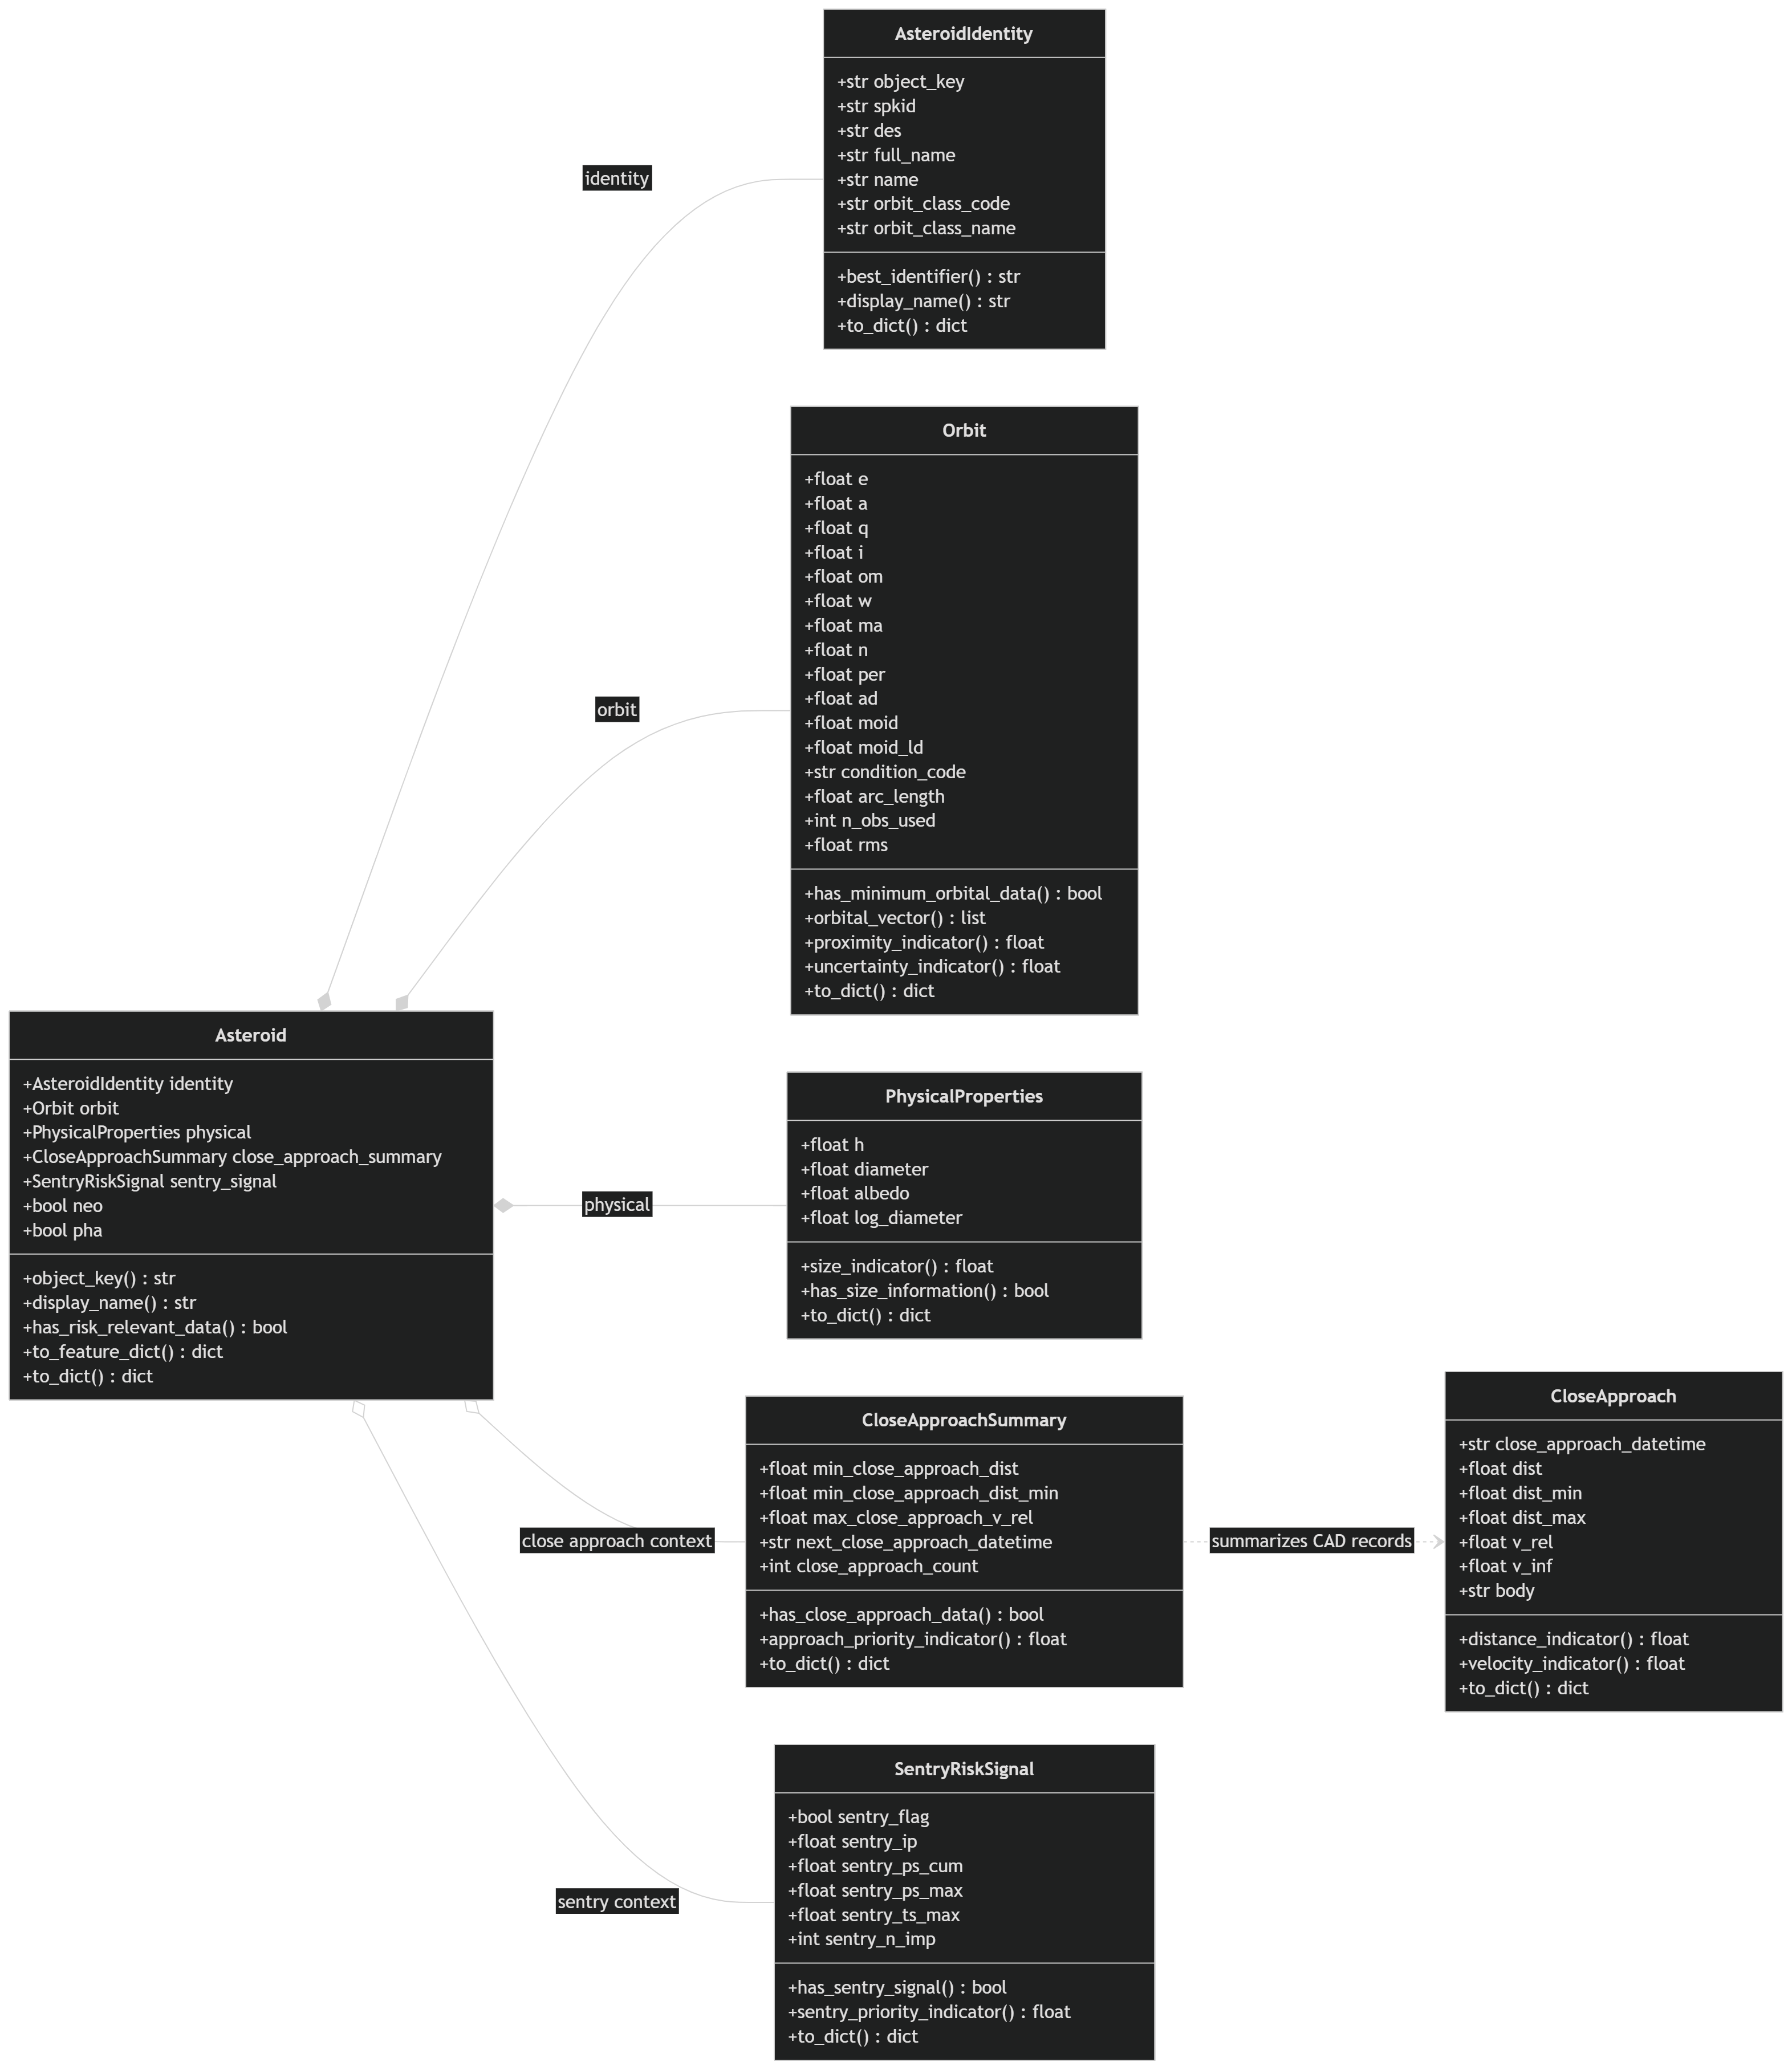
\includegraphics[width=0.95\textwidth]{figures/class-diagram-entities.png}
\caption{Diagrama UML de entidades puras del dominio.}
\end{figure}

El diagrama muestra \code{Asteroid} como agregado raíz y no como una división mecánica de columnas CSV. \code{AsteroidIdentity} concentra reglas de identificación porque \code{object\_key}, \code{spkid}, \code{des}, \code{full\_name} y \code{name} no tienen la misma estabilidad. \code{Orbit} encapsula elementos orbitales y señales de calidad; \code{PhysicalProperties} agrupa magnitud absoluta, diámetro, albedo y proxies de tamaño; \code{CloseApproach} representa un evento individual y \code{CloseApproachSummary} resume señales CAD útiles para score y frontend. \code{SentryRiskSignal} es opcional porque la mayoría de objetos no tiene señal Sentry en el snapshot local. La elección de composición sobre herencia profunda evita una taxonomía artificial: órbita, propiedades físicas, acercamientos y señal Sentry son partes del agregado, no subtipos de asteroide.

\section{Clases Principales}

{\footnotesize
\setlength{\tabcolsep}{3.5pt}
\begin{longtable}{>{\RaggedRight\arraybackslash}p{0.17\linewidth}>{\RaggedRight\arraybackslash}p{0.23\linewidth}>{\RaggedRight\arraybackslash}p{0.31\linewidth}>{\RaggedRight\arraybackslash}p{0.19\linewidth}}
\caption{Clases de dominio verificadas.}\\
\toprule
Clase & Archivo & Responsabilidad & Métodos principales\\
\midrule
\endfirsthead
\toprule
Clase & Archivo & Responsabilidad & Métodos principales\\
\midrule
\endhead
\code{Asteroid} & \filepath{src/neo_ange/domain/asteroid.py} & Agregado raíz con identidad, órbita, propiedades físicas, acercamientos, Sentry y etiquetas. & \code{object\_key}, \code{display\_name}, \code{has\_risk\_relevant\_data}, \code{to\_feature\_dict}, \code{to\_dict}.\\
\code{AsteroidIdentity} & \filepath{src/neo_ange/domain/identity.py} & Identificadores estables y nombre legible. & \code{best\_identifier}, \code{display\_name}, \code{to\_dict}.\\
\code{Orbit} & \filepath{src/neo_ange/domain/orbit.py} & Elementos orbitales y señales de calidad. & \code{has\_minimum\_orbital\_data}, \code{orbital\_vector}, \code{proximity\_indicator}, \code{uncertainty\_indicator}.\\
\code{PhysicalProperties} & \filepath{src/neo_ange/domain/physical.py} & Magnitud absoluta, diámetro, albedo y log diámetro. & \code{size\_indicator}, \code{has\_size\_information}, \code{to\_dict}.\\
\code{CloseApproach} & \filepath{src/neo_ange/domain/approach.py} & Un acercamiento individual. & \code{distance\_indicator}, \code{velocity\_indicator}, \code{to\_dict}.\\
\code{CloseApproachSummary} & \filepath{src/neo_ange/domain/approach.py} & Resumen CAD por objeto. & \code{has\_close\_approach\_data}, \code{approach\_priority\_indicator}.\\
\code{SentryRiskSignal} & \filepath{src/neo_ange/domain/sentry.py} & Señales Sentry disponibles. & \code{has\_sentry\_signal}, \code{sentry\_priority\_indicator}, \code{to\_dict}.\\
\code{AsteroidFactory} & \filepath{src/neo_ange/domain/factories.py} & Construye entidades desde filas gold, risk y simulación. & \code{from\_gold\_row}, \code{from\_risk\_row}, \code{many\_from\_dataframe}, \code{risk\_score\_from\_row}.\\
\code{GoldFeatureRepository}, \code{RiskScoreRepository}, \code{SimulationResultRepository} & \filepath{src/neo_ange/domain/repositories.py} & Aíslan lectura de Parquet y devuelven entidades. & \code{load\_dataframe}, \code{load\_asteroids}, \code{get\_by\_object\_key}, \code{top}.\\
\bottomrule
\end{longtable}
}

\section{Extractos Exactos}

\begin{lstlisting}[language=Python,caption={Extracto de asteroid.py}]
@dataclass(slots=True)
class Asteroid:
    """Domain aggregate containing risk-relevant asteroid state."""

    identity: AsteroidIdentity
    orbit: Orbit
    physical: PhysicalProperties
    close_approach_summary: CloseApproachSummary | None = None
    sentry_signal: SentryRiskSignal | None = None
    neo: bool | None = None
    pha: bool | None = None
\end{lstlisting}

\begin{lstlisting}[language=Python,caption={Extracto de factories.py}]
class AsteroidFactory:
    """Build domain objects from gold, risk-score, and simulation records."""

    @classmethod
    def from_gold_row(cls, row: dict[str, Any] | pd.Series) -> Asteroid:
        """Create an asteroid aggregate from a gold feature row."""
\end{lstlisting}

\chapter{Implementación Python por Archivo}

El inventario sintético se generó por inspección de archivos Python y se resume en la Tabla \ref{tab:inventory}. Para mantener legibilidad, no se incluyen archivos completos; se agrupan módulos públicos relevantes.

{\footnotesize
\setlength{\tabcolsep}{4pt}
\begin{longtable}{>{\RaggedRight\arraybackslash}p{0.22\linewidth}>{\RaggedRight\arraybackslash}p{0.26\linewidth}>{\RaggedRight\arraybackslash}p{0.42\linewidth}}
\caption{Inventario sintético de paquetes Python relevantes.}
\label{tab:inventory}\\
\toprule
Paquete o ruta & Clases o funciones principales & Responsabilidad técnica\\
\midrule
\endfirsthead
\toprule
Paquete o ruta & Clases o funciones principales & Responsabilidad técnica\\
\midrule
\endhead
\filepath{src/neo_ange/clients} & \code{BaseJPLClient}, \code{SBDBObjectClient}, \code{SBDBQueryClient}, \code{CloseApproachClient}, \code{SentryClient} & Encapsula las llamadas HTTP a las API públicas SBDB Object, SBDB Query, CAD y Sentry.\\
\filepath{src/neo_ange/services} & \code{BronzeStorage}, \code{SilverStorage}, \code{GoldStorage} & Resuelve rutas y persistencia local para capas bronze, silver y gold.\\
\filepath{src/neo_ange/etl} & \code{BronzeReader}, \code{SilverTransformers}, \code{GoldBuilder} & Normaliza JSON crudo, construye tablas silver y une features analíticas en gold.\\
\filepath{src/neo_ange/domain} & \code{Asteroid}, \code{Orbit}, \code{PhysicalProperties}, \code{CloseApproachSummary}, \code{SentryRiskSignal}, \code{AsteroidFactory}, repositorios & Modelo POO del dominio, mapeo desde filas gold y lectura orientada a objetos de artefactos Parquet.\\
\filepath{src/neo_ange/risk} & \code{RiskScorer}, \code{RiskCategoryAssigner}, \code{RiskExplanationService}, \code{RiskRankingService} & Calcula el Risk Priority Score, asigna categorías, genera explicaciones y rankings.\\
\filepath{src/neo_ange/simulation} & \code{MonteCarloEngine}, \code{PerturbationEngine}, \code{UncertaintySpec}, \code{SensitivityAnalyzer} & Propaga incertidumbre aproximada del score, recalcula escenarios y resume percentiles.\\
\filepath{src/neo_ange/orbital_simulation} & \code{OrbitalMonteCarloEngine}, \code{parse\_covariance\_payload}, \code{sample\_orbital\_clones}, \code{solve\_kepler} & Simula clones orbitales con covarianza o fallback heurístico y propagación kepleriana aproximada.\\
\filepath{src/neo_ange/ml} & \code{FeatureSetRegistry}, \code{RuleBasedPHABaseline}, \code{build\_estimator}, \code{run\_baseline\_experiments} & Entrena modelos tabulares, separa conjuntos de features y calcula métricas con auditoría de leakage.\\
\filepath{src/neo_ange/gnn} & \code{OrbitalGraphBuilder}, \code{OrbitalSimilarityCalculator}, \code{GraphBaselineRunner}, \code{GraphSAGEModel}, \code{GCNModel}, \code{GNNTrainer} & Construye grafo kNN, ejecuta baselines de grafo y entrena GNN si \code{torch-geometric} está disponible.\\
\filepath{src/neo_ange/evidence} & \code{ModelEvidenceBuilder}, predicciones, disagreement, model cards & Integra evidencia secundaria de modelos, tarjetas, inferencia completa/evaluación y desacuerdos.\\
\filepath{src/neo_ange/findings} & \code{FindingsBuilder} y generadores por módulo & Convierte artefactos analíticos en hallazgos interpretables para API y frontend.\\
\filepath{src/neo_ange/api} & \code{FastAPI}, routers de \code{health}, \code{risk}, \code{rankings}, \code{objects}, \code{simulations}, \code{orbital\_simulation}, \code{gnn}, \code{model\_evidence}, \code{findings}, \code{domain} & Expone resultados y ejecuciones bajo HTTP para el frontend React/Vite.\\
\filepath{src/neo_ange/pipelines} & \code{IngestionPipeline}, \code{ETLPipeline}, \code{RiskPipeline}, \code{SimulationPipeline}, \code{MLPipeline} & Orquesta flujos completos y manifiestos de ejecución.\\
\bottomrule
\end{longtable}
}


\chapter{Factories, Repositories y Servicios}

El patrón Factory centraliza creación de objetos. En lugar de repetir conversiones de \code{NaN}, strings vacíos, booleanos y floats en cada router, \code{AsteroidFactory} recibe filas limpias y produce entidades coherentes. Esto evita duplicación y permite modificar reglas de mapeo en un solo lugar.

El patrón Repository aísla persistencia. \code{GoldFeatureRepository} sabe dónde está \filepath{data/gold/neo_risk_features}; \code{RiskScoreRepository} sabe que la ruta preferida es \filepath{data/gold/risk_scores/risk_scores.parquet}; \code{SimulationResultRepository} sabe cómo leer resultados Monte Carlo. Los routers y servicios no manipulan rutas Parquet directamente cuando trabajan con dominio.

La capa de servicios coordina flujos: \code{RiskPipeline} calcula score, \code{SimulationPipeline} ejecuta Monte Carlo de score, \code{OrbitalSimulationService} ejecuta clones orbitales, \code{GNNExperimentRunner} construye grafo y modelos, y \code{ModelEvidenceBuilder} integra evidencia secundaria. Esta separación reduce acoplamiento entre ingestión, scoring, simulación, modelado, API y frontend.

\chapter{Risk Priority Score}

El \emph{Risk Priority Score} es un score experimental, reproducible y explicable. No es probabilidad oficial de impacto. Se implementa en \filepath{src/neo_ange/risk/scoring.py} y usa constantes de \filepath{src/neo_ange/risk/schemas.py}. La versión actual verificada es \code{risk-score-v0.1.0}.

\section{Fórmula}

Sean \(c_j \in [0,1]\) los componentes normalizados y \(w_j\) sus pesos. El score se calcula como:

\[
S = 100 \cdot \operatorname{clip}_{[0,1]}\left(
0.22c_{\text{physical}}+
0.25c_{\text{orbital}}+
0.18c_{\text{approach}}+
0.17c_{\text{sentry}}+
0.13c_{\text{uncertainty}}+
0.05c_{\text{quality}}
\right).
\]

{\footnotesize
\setlength{\tabcolsep}{4pt}
\begin{tabularx}{\linewidth}{>{\RaggedRight\arraybackslash}p{0.30\linewidth}>{\centering\arraybackslash}p{0.11\linewidth}Y}
\toprule
Componente & Peso & Variables usadas\\
\midrule
\code{physical\_risk\_component} & 0.22 & Diámetro, \code{h}, \code{log\_diameter}, \code{size\_proxy\_score}.\\
\code{orbital\_risk\_component} & 0.25 & MOID, MOID lunar, \code{inverse\_moid}, perihelio, excentricidad, inclinación.\\
\code{approach\_risk\_component} & 0.18 & Distancia mínima, velocidad relativa, conteo de acercamientos.\\
\code{sentry\_risk\_component} & 0.17 & \code{sentry\_flag}, presencia, probabilidad, Palermo, Torino, número de impactores virtuales.\\
\code{uncertainty\_risk\_component} & 0.13 & \code{condition\_code}, \code{rms}, arco de observación, observaciones usadas, proxy de incertidumbre.\\
\code{data\_quality\_component} & 0.05 & Incompletitud, arco corto y baja cantidad de observaciones.\\
\bottomrule
\end{tabularx}
}

Las categorías son: \code{low} para score menor a 20; \code{moderate} desde 20 hasta menor que 40; \code{elevated} desde 40 hasta menor que 60; \code{high} desde 60 hasta menor que 80; \code{critical} desde 80.

\begin{lstlisting}[language=Python,caption={Pesos exactos del score}]
DEFAULT_COMPONENT_WEIGHTS: dict[str, float] = {
    "physical_risk_component": 0.22,
    "orbital_risk_component": 0.25,
    "approach_risk_component": 0.18,
    "sentry_risk_component": 0.17,
    "uncertainty_risk_component": 0.13,
    "data_quality_component": 0.05,
}
\end{lstlisting}

\chapter{Score Simulation y Monte Carlo}

El Monte Carlo del score se implementa en \filepath{src/neo_ange/simulation}. Monte Carlo significa muestrear valores aleatorios bajo supuestos de incertidumbre y observar cómo cambia una salida; MCMC es una familia distinta orientada a construir cadenas de Markov para aproximar distribuciones posteriores. Este proyecto no usa MCMC.

\code{MonteCarloEngine.simulate\_object()} toma una fila base, construye \code{PerturbationConfig}, perturba variables base, recalcula features derivadas y vuelve a ejecutar \code{RiskScorer}. Las variables base verificadas en \code{BASE\_SCORE\_VARIABLES} incluyen \code{h}, \code{diameter}, \code{albedo}, \code{moid}, \code{moid\_ld}, distancias de acercamiento, velocidad, campos Sentry, \code{condition\_code}, \code{rms}, \code{arc\_length} y \code{n\_obs\_used}.

El motor distingue incertidumbre reportada, escala empírica desde el dataset y fallback heurístico. El resumen incluye media, desviación estándar, mínimo, percentiles 5/25/50/75/95, máximo, probabilidad de superar 60, probabilidad de superar 80, probabilidad de cambio de categoría, categoría base y categoría del percentil 95.

\begin{lstlisting}[language=Python,caption={Variables base de incertidumbre}]
BASE_SCORE_VARIABLES = [
    "h",
    "diameter",
    "albedo",
    "moid",
    "moid_ld",
    "min_close_approach_dist",
    "min_close_approach_dist_min",
    "max_close_approach_v_rel",
    "sentry_ip",
    "sentry_ps_cum",
    "sentry_ps_max",
    "sentry_ts_max",
    "condition_code",
    "rms",
    "arc_length",
    "n_obs_used",
]
\end{lstlisting}

En el snapshot verificado, \filepath{data/gold/simulation_results/score_uncertainty_results.parquet} contiene 221 filas y 107 objetos únicos. El resumen JSON reporta \code{fallback\_used\_count=10} y \code{formal\_uncertainty\_count=0}, lo cual confirma que las simulaciones no deben presentarse como incertidumbre física calibrada.

\chapter{Simulación Orbital Monte Carlo}

La simulación orbital se implementa en \filepath{src/neo_ange/orbital_simulation}. El servicio usa \code{n\_clones=300}, \code{horizon\_days=3650}, \code{time\_step\_days=10} y \code{random\_state=42} por defecto. Esos valores equilibran costo, resolución temporal y rapidez para API/frontend: diez años de horizonte con pasos de diez días da una exploración suficiente para visualización experimental, pero no sustituye efemérides oficiales.

\section{Covarianza y Fallback}

Una varianza mide dispersión de una variable. Una covarianza mide cómo dos variables cambian juntas. Una matriz de covarianza orbital describe incertidumbre conjunta entre elementos orbitales; si está disponible y es válida, permite muestrear clones con una normal multivariada más coherente que perturbar variables de manera independiente. El código parsea \code{covariance\_matrix\_json}, \code{covariance\_json} o \code{covariance\_matrix\_path}, valida simetría, diagonal, valores finitos y condición positiva semidefinida.

Cuando no hay covarianza usable, \code{OrbitalMonteCarloEngine} usa \code{heuristic\_fallback}. El score de incertidumbre combina \code{condition\_code}, \code{rms}, \code{arc\_length} y \code{n\_obs\_used} con pesos exactos 0.35, 0.25, 0.20 y 0.20.

\begin{lstlisting}[language=Python,caption={Fallback y parámetros orbitales}]
def simulate_object(
    self,
    row: dict[str, Any],
    n_clones: int = 300,
    horizon_days: int = 3650,
    time_step_days: int = 10,
    random_state: int | None = 42,
) -> dict[str, Any]:
\end{lstlisting}

\begin{lstlisting}[language=Python,caption={Peso de incertidumbre orbital}]
return float(
    np.clip(0.35 * condition_part + 0.25 * rms_part + 0.2 * arc_part + 0.2 * obs_part, 0, 1)
)
\end{lstlisting}

Los clones válidos son muestras con elementos finitos, semieje mayor positivo y excentricidad en rango físico. Los clones inválidos se cuentan en \code{invalid\_clone\_count}; los aceptados quedan en \code{valid\_clone\_count}. El resultado registra \code{simulation\_method}, \code{covariance\_available}, \code{covariance\_dimension}, \code{fallback\_reason}, \code{warning}, \code{cad\_validation\_available} y \code{cad\_validation\_error\_au}.

\section{Modelo Físico}

La propagación usa un modelo heliocéntrico aproximado de dos cuerpos, basado en elementos keplerianos clásicos \cite{bate1971fundamentals}. Para cada clon, se avanza la anomalía media con \(M(t)=M_0+n t\). La ecuación de Kepler es:

\[
M = E - e\sin(E).
\]

El código resuelve \(E\) con iteraciones de Newton-Raphson vectorizadas. Luego calcula posición en el plano orbital:

\[
x = a(\cos E - e), \qquad
y = a\sqrt{1-e^2}\sin E.
\]

Después rota al espacio 3D con \(w\), \(i\) y \(om\). La Tierra se aproxima como órbita circular de 1 AU. Para cada día del grid temporal se calcula la distancia euclidiana objeto-Tierra y se conserva la mínima por clon. Las métricas finales son media, desviación estándar, percentiles p05/p50/p95, día de acercamiento, \code{dispersion\_index} y \code{scenario\_category}. Las categorías verificadas en el código son \code{stable}, \code{variable}, \code{uncertain} y \code{needs\_review}.

La limitación física es deliberada: no hay modelo N-body, no hay efemérides oficiales, no hay perturbaciones planetarias precisas y no hay sistema de alerta. El objetivo es producir escenarios visuales y comparativos para la aplicación.

\chapter{Machine Learning Tabular}

Los modelos tabulares se implementan en \filepath{src/neo_ange/ml}. El objetivo verificado es \code{pha}. Los modelos disponibles son \code{DummyClassifier}, \code{LogisticRegression}, \code{RandomForestClassifier}, \code{HistGradientBoostingClassifier} y \code{RuleBasedPHABaseline}. La documentación y los reportes siguen las prácticas de scikit-learn \cite{sklearn_docs}.

El DummyClassifier con estrategia \code{most\_frequent} establece una línea base ingenua. La regresión logística modela:

\[
p(y=1\mid x)=\frac{1}{1+e^{-z}}, \qquad z=w^\top x+b.
\]

En el código usa \code{class\_weight="balanced"}, \code{max\_iter=1000} y \code{random\_state=42}. Random Forest combina árboles entrenados con bagging; el código usa \code{n\_estimators=100}, \code{min\_samples\_leaf=2}, \code{class\_weight="balanced"} y \code{n\_jobs=-1}. HistGradientBoosting usa boosting con \code{learning\_rate=0.08}, \code{max\_iter=100} y \code{random\_state=42}. El baseline rule-based marca PHA aproximado cuando \(\mathrm{moid} \le 0.05\) y \(h \le 22.0\).

\begin{lstlisting}[language=Python,caption={Parámetros exactos de modelos}]
if model_name == LOGISTIC_MODEL:
    return LogisticRegression(class_weight="balanced", max_iter=1000, random_state=random_state)
if model_name == RANDOM_FOREST_MODEL:
    return RandomForestClassifier(
        class_weight="balanced",
        n_estimators=100,
        min_samples_leaf=2,
        random_state=random_state,
        n_jobs=-1,
    )
\end{lstlisting}

Los feature sets verificados son \code{full\_features}, \code{definition\_features\_only}, \code{no\_definition\_features}, \code{orbital\_only}, \code{approach\_and\_quality} y \code{sentry\_related}. \code{full\_features} y \code{definition\_features\_only} pueden inflar métricas porque incluyen variables cercanas a la definición PHA. Por eso el proyecto reporta leakage y separa evidencia defensible.

\chapter{Métricas de ML}

La matriz de confusión contiene verdaderos positivos (TP), falsos positivos (FP), verdaderos negativos (TN) y falsos negativos (FN). Accuracy mide proporción total correcta, pero puede ocultar mal desempeño en clases minoritarias. Precision mide \(TP/(TP+FP)\), recall mide \(TP/(TP+FN)\), F1 combina precision y recall. ROC-AUC resume separación entre clases sobre umbrales; PR-AUC es especialmente útil con desbalance porque se enfoca en positivos.

El reporte \filepath{reports/model_evidence/model_evidence_summary.json} registra como mejor evidencia defensible a \code{graphsage} con feature set \code{graph}, PR-AUC 0.9760233191710436, F1 0.9316455696202532 y ROC-AUC 0.9923131504257332. Sin embargo, el reporte GNN actual \filepath{reports/gnn/gnn_summary.md} indica que \code{torch-geometric} no estuvo instalado y que GraphSAGE/GCN se omitieron en esa corrida. Esta diferencia se documenta como desalineación entre artefactos de evidencia y corrida GNN local. La conclusión honesta es que ML/GNN proporciona evidencia secundaria y debe interpretarse según el snapshot que produjo cada archivo.

\chapter{Grafo Orbital, GNN y Deep Learning}

Un grafo tiene nodos y aristas. En este proyecto cada nodo representa un objeto y cada arista representa similitud orbital kNN. \code{OrbitalSimilarityCalculator} selecciona features numéricas seguras, excluye identificadores y variables prohibidas, imputa medianas, escala con \code{StandardScaler}, calcula vecinos con distancia euclidiana y transforma distancia a similitud:

\[
\operatorname{similarity} = \frac{1}{1+\operatorname{distance}}.
\]

El parámetro real por defecto es \code{k=10}. En el snapshot actual, \filepath{data/gold/gnn_graph/nodes.parquet} contiene 1,000 nodos y \filepath{edges.parquet} contiene 6,955 aristas. El reporte \filepath{reports/findings/findings_summary.json} conserva una corrida de 4,000 nodos y 27,829 aristas; se mantiene como reporte existente, pero no se mezcla con el grafo actual.

Una red neuronal aprende representaciones a partir de entradas numéricas. Un embedding es una representación vectorial aprendida. Una GNN extiende esta idea a grafos mediante \emph{message passing}: cada nodo actualiza su representación usando información de sus vecinos. La analogía con CNN es que ambas explotan estructura local; la CNN usa vecindarios espaciales en una grilla, la GNN usa vecindarios definidos por aristas.

\filepath{src/neo_ange/gnn/models.py} define \code{GraphSAGEModel} y \code{GCNModel} si \code{torch-geometric} está disponible \cite{pytorch_geometric_docs}. Ambos usan \code{hidden\_channels=32}, \code{out\_channels=2} y \code{dropout=0.2}. \code{GNNTrainer} usa \code{epochs=100}, \code{patience=10}, optimizador Adam, \code{lr=0.01}, \code{weight\_decay=5e-4} y \code{random\_state=42}. Label Propagation aparece como baseline de grafo, no como deep learning; MLP aparece como baseline neuronal tabular o de features de grafo.

\begin{lstlisting}[language=Python,caption={Parámetros GNN}]
hidden_channels: int = 32,
out_channels: int = 2,
dropout: float = 0.2,

optimizer = torch.optim.Adam(model.parameters(), lr=0.01, weight_decay=5e-4)
\end{lstlisting}

\chapter{Model Evidence}

Model evidence integra predicciones, tarjetas de modelo, desacuerdos y conclusiones. La diferencia entre \code{model\_predictions\_eval} y \code{model\_predictions\_full} es central: eval corresponde a evaluación y full inference corresponde a inferencia extendida. El resumen verificado indica \code{prediction\_rows\_eval=5000}, \code{unique\_eval\_object\_keys=1000}, \code{prediction\_rows\_full=20000}, \code{unique\_full\_object\_keys=4000}, \code{coverage\_ratio=1.0} y \code{disagreement\_count=1363}.

El mejor modelo no se elige solamente por métrica bruta. El reporte identifica modelos con leakage sensible, por ejemplo \code{full\_features}, \code{definition\_features\_only} y \code{graph\_node\_features}. La mejor evidencia defensible evita variables demasiado cercanas a la definición PHA. En una entrega académica, esta separación demuestra criterio: una métrica perfecta puede ser menos útil si aprende una definición codificada en sus entradas.

\chapter{Findings}

Los findings convierten artefactos analíticos en conclusiones legibles. Se generan desde \filepath{src/neo_ange/findings} y leen risk scores, simulaciones, grafo, evidencia de modelos y dataset. El archivo \filepath{reports/findings/findings_summary.json} contiene 19 hallazgos y reporta 4,000 objetos, 982 PHA, 3,018 non-PHA, 18 objetos con señal Sentry, 37 objetos elevados o superiores, 335 filas de simulación de score, 10 filas de simulación orbital, 4,000 nodos de grafo y 27,829 aristas.

Ese reporte no coincide por completo con los Parquet actuales de \filepath{data/gold}, que tienen 1,000 filas en gold/risk y 1,000 nodos de grafo. Por tanto, los findings se documentan como resultado generado existente, no como descripción única del estado actual de todas las capas. Esta limitación es importante para reproducibilidad: antes de presentar métricas definitivas, debe regenerarse el pipeline completo o congelarse un snapshot consistente.

\chapter{API FastAPI}

FastAPI permite exponer rutas HTTP con validación Pydantic \cite{fastapi_docs}. La aplicación vive en \filepath{src/neo_ange/api/main.py}. Los routers verificados incluyen:

\begin{itemize}
  \item \code{health}: salud y estado de artefactos.
  \item \code{risk}: construcción de score, estado y explicaciones.
  \item \code{rankings}: rankings por score y categoría.
  \item \code{objects}: listado y perfil de objetos.
  \item \code{simulations}: Monte Carlo del score.
  \item \code{orbital\_simulation}: simulación orbital aproximada.
  \item \code{gnn}: estado, construcción de grafo, métricas y vecinos.
  \item \code{model\_evidence}: resumen, tarjetas, predicciones y desacuerdos.
  \item \code{findings}: hallazgos por módulo.
  \item \code{domain}: objeto en representación de agregado de dominio.
\end{itemize}

El backend se ejecuta en el puerto 8000 dentro de \filepath{docker-compose.yml} con \code{uvicorn neo\_ange.api.main:app --host 0.0.0.0 --port 8000}. El frontend consume la API mediante \code{VITE\_API\_BASE\_URL=http://127.0.0.1:8000}.

\chapter{Frontend React/Vite}

El frontend vive en \filepath{frontend}. Usa React, TypeScript y Vite \cite{react_docs,vite_docs}. Las páginas verificadas por rutas y archivos son \code{MissionControlPage}, \code{RiskRankingPage}, \code{AsteroidProfilePage}, \code{MonteCarloLabPage}, \code{OrbitalSimulationPage}, \code{GNNResearchLabPage}, \code{FindingsPage}, \code{MethodologyPage}, \code{ModelAndLeakageLabPage}, \code{PipelineMonitorPage} y \code{DomainExplorerPage}.

La consigna menciona páginas con nombres funcionales como Control Panel, Risk Ranking, Object Profile, Score Simulation, Orbital Simulation, Orbital Graph, Findings y Methodology. En el código actual esos conceptos existen con nombres de página equivalentes. El valor de la interfaz está en hacer navegables rankings, perfiles, simulaciones, evidencia, grafo y metodología sin obligar al usuario a leer Parquet o JSON directamente.

\chapter{Docker y Ejecución}

Docker empaqueta dependencias y servicios; Docker Compose levanta múltiples servicios desde un solo archivo \cite{docker_ubuntu,docker_debian,docker_compose}. El \filepath{docker-compose.yml} define:

\begin{itemize}
  \item \code{app}: backend FastAPI en \code{http://127.0.0.1:8000}, con volúmenes \code{data}, \code{reports} y \code{artifacts}.
  \item \code{frontend}: frontend servido en \code{http://127.0.0.1:5174}, construido con \code{Dockerfile.frontend}.
\end{itemize}

La primera construcción puede tardar porque descarga imágenes, instala Python, PySpark, scikit-learn, dependencias científicas, Node y paquetes frontend. También puede tardar la primera generación de reportes o carga de datos por el volumen de artefactos.

\chapter{Resultados Obtenidos}

\section{Consistencia y Alcance del Snapshot Verificado}

La Tabla \ref{tab:results} separa tres tipos de evidencia: artefactos Parquet verificados directamente en el checkout actual, reportes JSON/Markdown existentes y resultados heredados de corridas ampliadas. Esta separación evita mezclar como si fueran un único estado definitivo los 1,000 objetos presentes en \filepath{data/gold} con los 4,000 objetos que aparecen en algunos reportes de evidencia y findings.

{\footnotesize
\setlength{\tabcolsep}{4pt}
\begin{tabularx}{\linewidth}{>{\RaggedRight\arraybackslash}p{0.28\linewidth}>{\RaggedRight\arraybackslash}p{0.24\linewidth}>{\RaggedRight\arraybackslash}X}
\toprule
Artefacto verificado & Resultado observado & Interpretación\\
\midrule
\filepath{data/gold/neo_risk_features} & 1,000 filas; 1,000 \code{object\_key}; 280 PHA; 720 non-PHA; 2 con \code{sentry\_flag} & Snapshot gold tabular actual leído con \code{pandas.read\_parquet}.\\
\filepath{data/gold/risk_scores} & 1,000 filas; categorías: 70 \code{low}, 909 \code{moderate}, 21 \code{elevated} & Ranking actual de score local; máximo 47.271572 para \code{20152637}.\\
\filepath{reports/model_evidence/model_predictions_full.parquet} & 20,000 filas; 4,000 \code{object\_key} únicos & Inferencia completa de evidencia de modelos; no coincide en cobertura con el gold actual de 1,000 filas.\\
\filepath{reports/model_evidence/model_predictions_eval.parquet} & 5,000 filas; 1,000 \code{object\_key} únicos & Predicciones de evaluación sobre 1,000 objetos.\\
\filepath{data/gold/simulation_results/score_uncertainty_results.parquet} & 221 filas; 107 \code{object\_key} únicos; versión \code{risk-score-uncertainty-v0.2.0} & Resultados persistidos de Monte Carlo del score; no todos los objetos tienen simulación guardada.\\
\filepath{reports/orbital_simulation/orbital_simulation_summary.json} & 10 filas reportadas; categorías: 1 \code{stable}, 1 \code{variable}, 5 \code{uncertain}, 3 \code{needs\_review} & Resumen generado previamente.\\
\filepath{data/gold/orbital_simulation/orbital_monte_carlo_results.parquet} & 1 fila actual; objeto \code{20089958}; categoría orbital \code{variable} & Parquet actual más reducido que el resumen JSON; se documenta como desalineación de artefactos.\\
\filepath{data/gold/gnn_graph/nodes.parquet} y \filepath{edges.parquet} & 1,000 nodos; 6,955 aristas & Grafo kNN actual construido con \code{k=10}.\\
\filepath{reports/findings/findings_summary.json} & Reporta 4,000 objetos, 982 PHA, 3,018 non-PHA, 27,829 aristas y 37 \code{elevated} & Hallazgos generados contra un snapshot anterior o ampliado; se conservan como reporte existente, no como estado único del gold actual.\\
\bottomrule
\end{tabularx}
}


\chapter{Guía de Instalación Linux Desde Cero}

La instalación objetivo es Ubuntu, Debian o Linux Mint. Linux Mint usa base Ubuntu, por lo que se usa el repositorio Docker de Ubuntu con el codename de Ubuntu subyacente cuando corresponda.

\section{Instalación Completa: Copiar y Pegar}

\begin{lstlisting}[language=bash]
sudo apt-get update
sudo apt-get upgrade -y
sudo apt-get install -y git curl ca-certificates gnupg lsb-release

sudo install -m 0755 -d /etc/apt/keyrings
if [ -f /etc/linuxmint/info ]; then
  . /etc/os-release
  UBUNTU_CODENAME="${UBUNTU_CODENAME:-$(. /etc/linuxmint/info && echo "$UBUNTU_CODENAME")}"
  curl -fsSL https://download.docker.com/linux/ubuntu/gpg | sudo gpg --dearmor -o /etc/apt/keyrings/docker.gpg
  echo "deb [arch=$(dpkg --print-architecture) signed-by=/etc/apt/keyrings/docker.gpg] https://download.docker.com/linux/ubuntu ${UBUNTU_CODENAME} stable" | sudo tee /etc/apt/sources.list.d/docker.list > /dev/null
elif . /etc/os-release && [ "$ID" = "debian" ]; then
  curl -fsSL https://download.docker.com/linux/debian/gpg | sudo gpg --dearmor -o /etc/apt/keyrings/docker.gpg
  echo "deb [arch=$(dpkg --print-architecture) signed-by=/etc/apt/keyrings/docker.gpg] https://download.docker.com/linux/debian $(. /etc/os-release && echo "$VERSION_CODENAME") stable" | sudo tee /etc/apt/sources.list.d/docker.list > /dev/null
else
  curl -fsSL https://download.docker.com/linux/ubuntu/gpg | sudo gpg --dearmor -o /etc/apt/keyrings/docker.gpg
  echo "deb [arch=$(dpkg --print-architecture) signed-by=/etc/apt/keyrings/docker.gpg] https://download.docker.com/linux/ubuntu $(. /etc/os-release && echo "${UBUNTU_CODENAME:-$VERSION_CODENAME}") stable" | sudo tee /etc/apt/sources.list.d/docker.list > /dev/null
fi
sudo chmod a+r /etc/apt/keyrings/docker.gpg
sudo apt-get update
sudo apt-get install -y docker-ce docker-ce-cli containerd.io docker-buildx-plugin docker-compose-plugin
sudo usermod -aG docker "$USER"
newgrp docker

docker --version
docker compose version
docker run --rm hello-world

git clone https://github.com/LiamSalazar/NEO-Angele-Risk-Lab.git
cd NEO-Angele-Risk-Lab
docker compose up -d --build app frontend
docker compose ps
curl http://127.0.0.1:8000/health
curl http://127.0.0.1:8000/status
\end{lstlisting}

URL frontend: \url{http://127.0.0.1:5174}. API: \url{http://127.0.0.1:8000}.

\section{Comandos Rápidos con Docker ya Instalado}

\begin{lstlisting}[language=bash]
git clone https://github.com/LiamSalazar/NEO-Angele-Risk-Lab.git
cd NEO-Angele-Risk-Lab
docker compose up -d --build app frontend
curl http://127.0.0.1:8000/health
docker compose down
\end{lstlisting}

\chapter{Solución de Problemas Comunes}

{\footnotesize
\setlength{\tabcolsep}{4pt}
\begin{longtable}{>{\RaggedRight\arraybackslash}p{0.28\linewidth}>{\RaggedRight\arraybackslash}p{0.64\linewidth}}
\caption{Problemas comunes y comandos reales.}\\
\toprule
Problema & Comando o acción\\
\midrule
\endfirsthead
\toprule
Problema & Comando o acción\\
\midrule
\endhead
Permisos de Docker & Ejecutar \code{sudo usermod -aG docker "\$USER"} y luego \code{newgrp docker}; si sigue fallando, cerrar sesión y entrar de nuevo.\\
Solo levantó frontend y no backend & \code{docker compose ps -a}; \code{docker compose logs -f app}; \code{docker compose up -d app frontend}.\\
Se canceló \code{docker compose build} & Repetir \code{docker compose build app frontend} y luego \code{docker compose up -d app frontend}.\\
\code{image not found} & Reconstruir con \code{docker compose build --no-cache app frontend}.\\
Puerto ocupado & Revisar procesos con \codepath{sudo ss -ltnp | grep ':8000|:5174'} o cambiar puertos en \code{docker-compose.yml}.\\
Backend no responde & \code{docker compose logs -f app}; validar \code{curl http://127.0.0.1:8000/health}.\\
\code{model\_predictions\_full.parquet} no existe & Ejecutar \code{docker compose exec -T app python -m neo\_ange.cli model-evidence build}.\\
Evidence no cubre 4,000 \code{object\_key} & Verificar \code{reports/model\_evidence/model\_evidence\_summary.json} y regenerar evidencia después de regenerar gold/risk.\\
Reports viejos & Reconstruir pipelines: \code{python -m neo\_ange.cli risk build}, \code{python -m neo\_ange.cli model-evidence build}, \code{python -m neo\_ange.cli findings build}.\\
Logs & \code{docker compose logs -f app}; \code{docker compose logs -f frontend}.\\
Reconstrucción de app & \code{docker compose build app}; \code{docker compose up -d --no-build app frontend}.\\
Validación de data/gold y reports & Usar el bloque Python de validación incluido en la sección siguiente.\\
\bottomrule
\end{longtable}
}

\begin{lstlisting}[language=bash,caption={Validación rápida dentro del contenedor}]
docker compose exec -T app python - <<'EOF'
import pandas as pd
from pathlib import Path

paths = [
    "data/gold/neo_risk_features",
    "data/gold/risk_scores",
    "reports/model_evidence/model_predictions_full.parquet",
]
for p in paths:
    path = Path(p)
    print("\n===", p, "===")
    print("exists:", path.exists())
    if path.exists():
        df = pd.read_parquet(path)
        print("rows:", len(df))
        if "object_key" in df.columns:
            print("unique_object_key:", df["object_key"].astype(str).nunique())
        print("columns:", list(df.columns)[:30])
EOF
\end{lstlisting}

\chapter{Validación}

Comandos de validación del backend:

\begin{lstlisting}[language=bash]
python -m pytest
python -m ruff check .
python -m black --check .
python -m neo_ange.cli risk build
python -m neo_ange.cli model-evidence build
python -m neo_ange.cli findings build
\end{lstlisting}

Comandos de validación del frontend:

\begin{lstlisting}[language=bash]
cd frontend
npm install
npm run lint
npm run test
npm run build
\end{lstlisting}

Comandos de validación con Docker:

\begin{lstlisting}[language=bash]
docker compose ps
curl http://127.0.0.1:8000/health
curl http://127.0.0.1:8000/status
\end{lstlisting}

La validación documental corresponde a Overleaf: este archivo está preparado para pdfLaTeX y BibTeX, sin \code{minted} y sin \code{shell-escape}. La validación de ejecución del sistema es distinta: en la computadora usada para preparar esta revisión, \code{docker} no está instalado o no está en PATH, por lo que no se pudo ejecutar \code{docker compose up}. Si no existe LaTeX local, la compilación debe realizarse en Overleaf con \filepath{latex_doc/main.tex} como archivo principal.

\chapter{Limitaciones}

Neo Angele Risk Lab no es un sistema oficial de alerta. No reemplaza NASA/JPL, CNEOS, Sentry ni análisis orbital profesional. El Risk Priority Score es experimental y depende del snapshot local. La simulación orbital usa un modelo de dos cuerpos, Tierra circular de 1 AU, resolución temporal fija y no incluye N-body ni efemérides oficiales. La covarianza no siempre está disponible; cuando falta, el fallback heurístico se marca explícitamente.

ML y GNN son evidencia secundaria. Existe riesgo de leakage cuando se usan variables cercanas a la definición PHA. Los reportes actuales no están perfectamente alineados: algunos artefactos resumen 4,000 objetos y otros Parquet actuales contienen 1,000. La cobertura CAD también es limitada por consulta y snapshot. Antes de una presentación numérica definitiva debe regenerarse todo el pipeline en una sola corrida o congelarse una versión consistente de datos y reportes.

\chapter{Conclusiones}

El proyecto logra integrar adquisición de datos, ETL con PySpark, modelo de dominio POO, scoring explicable, simulación Monte Carlo, simulación orbital aproximada, ML tabular, grafo orbital, evidencia secundaria, API FastAPI, frontend React/Vite, reportes y documentación. Demuestra competencias de arquitectura, ingeniería de datos, programación orientada a objetos, análisis de incertidumbre, machine learning, diseño de interfaces y reproducibilidad.

Su principal aporte académico es mostrar cómo construir una aplicación analítica completa sin ocultar límites: el score no es probabilidad oficial, la simulación no es efeméride profesional, y los modelos no sustituyen criterios de dominio. Esa honestidad técnica fortalece la entrega porque permite entender qué hace el sistema, qué no hace y por qué sus resultados deben interpretarse como laboratorio experimental.

\appendix

\chapter{Apéndice A: Comandos CLI}

\begin{lstlisting}[language=bash]
python -m neo_ange.cli info
python -m neo_ange.cli etl run-all
python -m neo_ange.cli risk build
python -m neo_ange.cli risk top --limit 20
python -m neo_ange.cli simulate batch --limit 50 --n-simulations 500
python -m neo_ange.cli orbital-sim batch --limit 50 --n-clones 300
python -m neo_ange.cli gnn build-graph
python -m neo_ange.cli gnn run
python -m neo_ange.cli model-evidence build
python -m neo_ange.cli findings build
\end{lstlisting}

\chapter{Apéndice B: Diagramas Mermaid Fuente}

El repositorio contiene los siguientes diagramas fuente: \filepath{docs/diagrams/system_architecture.mmd}, \filepath{docs/diagrams/data_pipeline_bronze_silver_gold.mmd}, \filepath{docs/diagrams/class_diagram_entities.mmd}, \filepath{docs/diagrams/class_diagram_system.mmd}, \filepath{docs/diagrams/risk_scoring_flow.mmd}, \filepath{docs/diagrams/score_monte_carlo_flow.mmd}, \filepath{docs/diagrams/orbital_simulation_flow.mmd}, \filepath{docs/diagrams/ml_model_evidence_flow.mmd}, \filepath{docs/diagrams/gnn_orbital_graph_flow.mmd}, \filepath{docs/diagrams/api_frontend_sequence.mmd} y \filepath{docs/diagrams/final_app_navigation.mmd}. Este documento incluye la imagen UML disponible y referencia los Mermaid como fuentes auditables.

\cleardoublepage
\phantomsection
\addcontentsline{toc}{chapter}{Bibliografía}
\bibliographystyle{apalike}
\bibliography{references}

\end{document}
